% Options for packages loaded elsewhere
\PassOptionsToPackage{unicode}{hyperref}
\PassOptionsToPackage{hyphens}{url}
%
\documentclass[
]{article}
\usepackage{lmodern}
\usepackage{amssymb,amsmath}
\usepackage{ifxetex,ifluatex}
\ifnum 0\ifxetex 1\fi\ifluatex 1\fi=0 % if pdftex
  \usepackage[T1]{fontenc}
  \usepackage[utf8]{inputenc}
  \usepackage{textcomp} % provide euro and other symbols
\else % if luatex or xetex
  \usepackage{unicode-math}
  \defaultfontfeatures{Scale=MatchLowercase}
  \defaultfontfeatures[\rmfamily]{Ligatures=TeX,Scale=1}
\fi
% Use upquote if available, for straight quotes in verbatim environments
\IfFileExists{upquote.sty}{\usepackage{upquote}}{}
\IfFileExists{microtype.sty}{% use microtype if available
  \usepackage[]{microtype}
  \UseMicrotypeSet[protrusion]{basicmath} % disable protrusion for tt fonts
}{}
\makeatletter
\@ifundefined{KOMAClassName}{% if non-KOMA class
  \IfFileExists{parskip.sty}{%
    \usepackage{parskip}
  }{% else
    \setlength{\parindent}{0pt}
    \setlength{\parskip}{6pt plus 2pt minus 1pt}}
}{% if KOMA class
  \KOMAoptions{parskip=half}}
\makeatother
\usepackage{xcolor}
\IfFileExists{xurl.sty}{\usepackage{xurl}}{} % add URL line breaks if available
\IfFileExists{bookmark.sty}{\usepackage{bookmark}}{\usepackage{hyperref}}
\hypersetup{
  hidelinks,
  pdfcreator={LaTeX via pandoc}}
\urlstyle{same} % disable monospaced font for URLs
\usepackage[margin=1in]{geometry}
\usepackage{graphicx,grffile}
\makeatletter
\def\maxwidth{\ifdim\Gin@nat@width>\linewidth\linewidth\else\Gin@nat@width\fi}
\def\maxheight{\ifdim\Gin@nat@height>\textheight\textheight\else\Gin@nat@height\fi}
\makeatother
% Scale images if necessary, so that they will not overflow the page
% margins by default, and it is still possible to overwrite the defaults
% using explicit options in \includegraphics[width, height, ...]{}
\setkeys{Gin}{width=\maxwidth,height=\maxheight,keepaspectratio}
% Set default figure placement to htbp
\makeatletter
\def\fps@figure{htbp}
\makeatother
\setlength{\emergencystretch}{3em} % prevent overfull lines
\providecommand{\tightlist}{%
  \setlength{\itemsep}{0pt}\setlength{\parskip}{0pt}}
\setcounter{secnumdepth}{-\maxdimen} % remove section numbering
% https://github.com/rstudio/rmarkdown/issues/337
\let\rmarkdownfootnote\footnote%
\def\footnote{\protect\rmarkdownfootnote}

% https://github.com/rstudio/rmarkdown/pull/252
\usepackage{titling}
\setlength{\droptitle}{-2em}

\pretitle{\vspace{\droptitle}\centering\huge}
\posttitle{\par}

\preauthor{\centering\large\emph}
\postauthor{\par}

\predate{\centering\large\emph}
\postdate{\par}

\date{}

\begin{document}

\hypertarget{actors-motive}{%
\section{An Unfurling Crisis}\label{actors-motive}}

When 10 million Americans---1 of every 20 adults---lost their
homes,\footnote{Martin and Niedt, \emph{Foreclosed America}.} it was
clear that homeowners needed an intervention. When Countrywide, which
two years earlier had serviced 20\% of the mortgages in the United
States,\footnote{Seabrooke, \emph{The Politics of Housing Booms and
  Busts}.} collapsed in July 2008, it was clear that the real estate
industry needed to change. When cities and counties around California,
Florida, Nevada, and Arizona trembled at a declining tax base, it was
clear that municipalities needed a break. Yet, none of these actors
wielded much power in the response to the subprime mortgage crisis.
Unlike the Great Depression, homeowners barely organized their political
power and financial institutions imposed very modest debtor-relief
programs. Additionally, the long-term trend of municipal disinvestment
emphasized the need to remove neighborhood blight instead of create or
subsidize housing.

In reponse, the Housing and Economic Recovery Act of 2008 (HERA)
authorized the Department of Housing and Urban Development (HUD) to
distribute \$3.9 billion to state and local governments for the purchase
and repair of foreclosed properties.\footnote{Pelosi, ``Text - H.R.3221
  - 110th Congress (2007-2008).''} This program, later termed the
Neighborhood Stabilization Program (NSP), is my focus. In purchasing,
repairing, and in most cases reselling foreclosed properties, the NSP
sought to mitigate the effects of foreclosures on their surroundings.
Primarily, foreclosures tear people from their homes. On top of this
comes the stigma of being a ``deadbeat''\footnote{Dayen, \emph{Chain of
  Title}.} and mounds of fees---legal, cancellation,
transportation-related. But once homeowners have been forced out, the
neighborhood and municipality bear the financial weight of that
foreclosure.

To nearby homeowners, foreclosures cost \$159,000 on average in
decreased property values.\footnote{Immergluck, \emph{Foreclosed}, 151.}
To the city or county that envelops the property, it costs around
\$50,000 for the legal and construction work to demolish and resell a
vacant lot, parcels which tend to drop property values even
further.\footnote{Indiviglio, ``The Housing Stabilization Program You
  Haven't Heard About.''} When property values drop, a home's
{[}apparent{]} equity drops too. This figure, estimated constantly by
market research firms such as Zillow and appraised periodically by
taxing authorities, determines to a large extent the wealth and
borrowing power of homeowners. If the value of an already-mortgaged home
rises, homeowners can refinance. While refinancing most often takes
advantage of lower interest rates or decreased principal amounts to
reduce monthly payments, refinancing was used by in the lead up to the
subprime mortgage crisis instead to finance renovations, service debts
(eg. student, credit card, and car loans), or cash out. Lending
institutions willingly converted apparent value into real value, and as
long as home values crept up, refinancing was viable. This use of
refinancing reflected a shift in how Americans approached housing, from
the home as an utterly private good, to the home as an asset. Homes
stand increasingly in the position of pension plans and 401ks; a wise
move can transform forty years into four-hundred thousand dollars.

These wise moves seemd to occur constantly from September 1992 until
March 2006. As @ref(fig:caseshiller) shows, the intervening 14 years
never once saw a drop in the industry's standard home-price metric, the
Case-Shiller U.S. National Home Price Index. As prices rose, homeowners
refinanced, effectively paying back the first mortgage while taking out
the second. To investors in mortgage-backed securities (MBS),
pre-payment from refinancing is usually seen as a risk, but constant and
predictable refinance added to the safety of securitization, playing
into investors risk-reward calculus. But when prices fell---or even
flatlined---this safety evaporated. Without the increased {[}apparent{]}
home equity, refinancing did nothing. Falling prices thus meant
homeowners were saddled with their current mortgage, often one whose
interest rates reset after two years, climbing an interest-rate
staircase for the next 28 years. Atop the interest payments, living
expenses (such as other debts) piled on to borrowers, where previously
refinancing had arrived to supplement existing income with cash. Falling
prices meant homeowners chose among food, water, and shelter, if they
had enough income for that to even be a decision.

\begin{figure}

{\centering 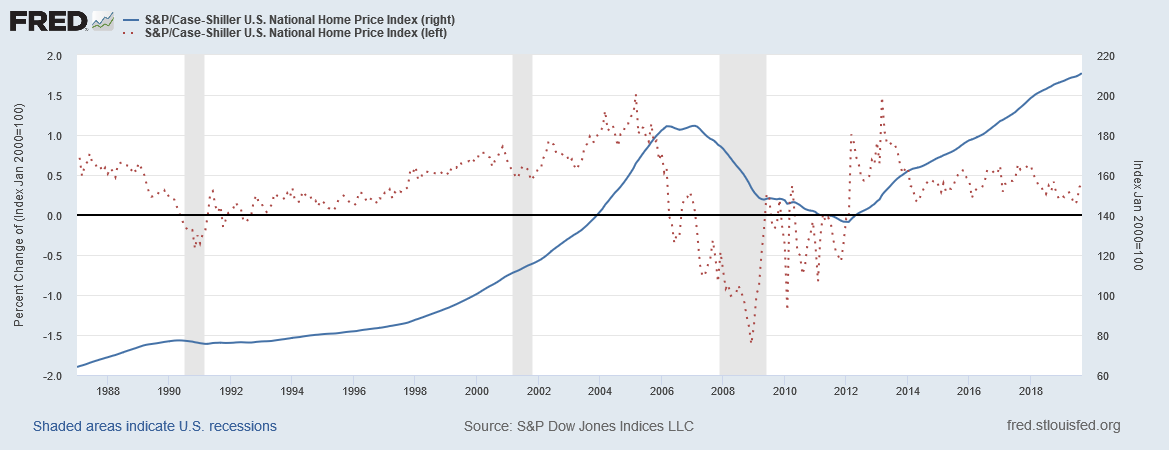
\includegraphics[width=0.9\linewidth]{figure/caseshiller_1990_2018} 

}

\caption{Price (right axis) and growth (left axis) of the Case-Shiller Home Price Index, adjusted for seasonal price fluctuations.}\label{fig:caseshiller}
\end{figure}

These factors make homeowners \emph{very} sensitive to falling or
stagnant home prices. In their sensitivity, they may have voted for
parties, candidates, and policies they believed would drive up home
prices, such as property tax cuts, musucular code enforcement, and
spacious zoning regulations. Each of these policies reduces the
resources available for non-homeowners, pitting homeowners against
renters, the homeless, and anyone else without a direct financial stake
in the asset. For example, tax cuts, take they the form of
directly-decreased property taxes or the homeowner tax credit, reduce
the monies available to fund public goods. In the United States, party
ideology also ties higher taxes with explicitly redistributive policies,
though Democrats and Republicans archetypically differ as to whether
high taxes--more redistribution is good or bad. The rigidity of these
ideologies rationalizes the fear that rents extracted from higher
taxation will not return to the homeowners. Circling back to the
original home-price dynamic, higher home values fund greater
consumption, while lower property values and higher taxes (as they
always have) limit homeowners' capacities to spend, an activity
Americans very much enjoy.

When prices rose, creditor and debtor interests laid at some angle,
intersecting in the particular case of safe, two-year refinancing, but
divergent in the general case of refinancing that took advantage of
lower interest rates. On the other hand, falling housing prices
conformed the immediate interests of creditors and debtors to one
another, since delinquency and default eliminated any chance of
extracting further rents. Fears of a debt spiral triggered by falling
home prices also beset cities,\footnote{Muro, ``Fiscal Challenges Facing
  Cities.''} though there is some doubt that those fears were
justified.\footnote{Gross et al., ``The Local Squeeze''; Lutz, Molloy,
  and Shan, ``The Housing Crisis and State and Local Government Tax
  Revenue.''} With these interests in syzygy, why didn't homeowners,
investors, or cities assert solutions, even ones that were done chiefly
in their own interest? I argue in this chapter first that homeowners
remained quiet due to changes in the foreclosure process from the Great
Depression, the differential character of housing versus farming, and
narratives about mortgage debtors. Second, the incongruity---spurred by
the demise of savings and loans---between incentives for principals in
mortgage-backed securities and agents tasked with servicing the
underlying mortgages, along with fraudulent mortgage transfers, resulted
in foreclosures that may have otherwise been unwanted by creditors.
Third, I point to municipal disinvestment and the trajectory of the
Commerce Clause as reasons why cities were unable to handle mass
foreclosures. This critique I believe to be sufficient, though by no
means necessary, to explaining why each was functionally barred from
substantial action.

This argument functions dual purposes. First, it justifes the motives of
actors external to the creation of the Neighborhood Stabilization
Program, to which internal actors, such as George W. Bush and members of
Congress, responded. Second, it offers a story about why external actors
may not have acted decisively. Readers should come away from this
chapter understanding why federal foreclosure relief programs were
necessary.

\hypertarget{homeowners}{%
\subsection{Why Homeowners were Unable to Organize}\label{homeowners}}

Reasons for the powerlessness of anti-foreclosure organizing can be
shown through comparison with the most successful anti-foreclosure
campaigns of the Great Depression. Legislative movements require a base
of public opinion and support, a mouthpiece through which opinion can be
articulated, and an powerful audience to hear those articulated opinions
and demands. Foreclosed housing's base of public opinion and support was
attenuated by geographic particularities of subprime mortgages which
limited fora for communication, both internally and externally. In
addition, the organizers' audience was blocked partially by other
demands, including the presence of mortgage servicers. The Great
Depression, however, saw these factors come together in the Midwest,
where farms were physically parched and thus, financially underwater.
Farmers were positioned similar to homeowners who adopted cash-out
refinancing in that they relied on their land for its income. However,
farmers in the Great Depression differed from early 2000s subprime
borrowers in that farming did not \emph{supplement} wage income, it
\emph{replaced} wage incomes. In addition, access to government and
stark differences in media portrayal combined with the larger impact of
farm foreclosures to drive organizing that led to 27 states enacting
\emph{per se} or \emph{de facto} moratoria on foreclosures.\footnote{Wheelock,
  ``Changing the Rules,'' 537.} The lack of such conditions pitched the
struggle for foreclosure legislation in the subprime mortgage crisis to
a severe angle.

The most important differentiator between the foreclosure crisis in the
Great Depression and that which preceded the Great Recession was the
outsize effect of farm foreclosures. Farms were both the workplace and
home of farmers. Unlike the foreclosure crisis in the 2000s, losing a
home implied losing a job, though that job could be lost in other ways
(drought, crop disease, low prices). This fact raised the stakes for
farmers to plead for relief and enlarged the macroeconomic worries with
which politicians were just beginning to grapple. Of the 100,000 farmers
who lost their farms each year between 1926 and 1940,\footnote{Alston,
  ``Farm Foreclosures in the United States During the Interwar Period.''}
the Midwest saw the highest concentrations. @ref(fig:wheelock-farms)
shows the high concentration in Minnesota, Iowa, and the Dakotas, and
the lesser concentration all around the Midwest. In 1933, by far the
worst year for farm mortgages, failure rates topped 3.7\%; during the
rest of 1926-1940, rates were often above 1.5\%.\footnote{Wheelock,
  ``Changing the Rules,'' 571.} By contrast, U.S. residential
foreclosures reached 1.8\% in 2008, the worst year of the mortgage
crisis.(REFRENCE NEEDED) In part, this is a denominator effect: the 50\%
down payments and double-digit interest rates caused fewer mortgages to
be demanded in the Great Depression. In large part, however, the
differences between farms and homes accounted for the scale.

\begin{figure}

{\centering \includegraphics[width=0.9\linewidth]{figure/wheelock} 

}

\caption{Figure taken from @wheelockChangingRulesState2008}\label{fig:wheelock-farms}
\end{figure}

The geography of farmland created several features that made easier mass
organizing. Lower population densities meant that fewer people exercised
political power over a fixed-size jurisdiction, when compared to a
densely-populated district. While this feature could not have played
into U.S. Congressional politics, which are apportioned by population,
it could make collusion easier in counties. Organization at the county
level was important in the Great Depression, because foreclosed
properties were sold by sheriffs, elected county officials.\footnote{Fliter
  and Hoff, \emph{Fighting Foreclosure}.} Compounding the numerical ease
of collusion was the congruency of interests. While farms produce a
variety of crops, soil and climate particularities combine with federal
agriculture policy to homogenize production locally. In other words,
Tobler's first law of geography holds: ``everything is related to
everything else, but near things are more related than distant
things.''\footnote{Tobler, ``A Computer Movie Simulating Urban Growth in
  the Detroit Region,'' 236.} In conversation with the realities of the
foreclosure crisis in the 2000s, two conclusions---one ecological, the
other sociological---emerge.

On the side of ecology, crop failures occurred in conjunction with
nearby farms. The same climate or disease that killed a neighbor's crops
could not be stopped at the property line. Farmers in the Great
Depression shared this feature with homeowners in the mortgage crisis:
lowered property values on one side would spillover to the other side.
For both populations, spatial correlations were imperfect, as some
farmers planted different crops and some foreclosures occurred among
conservative borrowers or wholly-owned homes, but the spillover effect
matters.\footnote{DeFusco et al., ``The Role of Price Spillovers in the
  American Housing Boom.''} Falling property values decreased the value
of neighboring properties, deepening the mortgage crisis for farmers in
the Depression and homeowners before the Recession. The conditions of
localized, severe economic distress existed in both eras.

But this comparison did not exist between the sociological features of
farming and housing. Farming the same crops entails some degree of
visiting the same market, buying the same tools, and asking the same
people for advice. Farmers met their neighbors whether they liked them
or not, creating a forum to talk shop with nearby people who shared
interests. The simple fact of homeownership, however, tends to signify
income, but little else, and the larger populations of suburbs facing
home foreclosures meant more social and cultural institutions among
which residents could choose. The higher density and absolute size of
the suburbs separated struggling homeowners from each other, while the
lack of farming meant that---even if they had bumped shoulders---their
mortgage finances were less likely to be topics of discussion. While the
suburban quality of foreclosures in the recent mortgage crisis could
have drawn homeowners closer together through their homeowner
association (HOA), HOAs were insignificant bulwarks against nearby
foreclosures.\footnote{Cheung, Cunningham, and Meltzer, ``Do Homeowners
  Associations Mitigate or Aggravate Negative Spillovers from
  Neighboring Homeowner Distress?'' 87.} And more to the point of
homeowner behavior, HOA fees were some of the first payments to stop
once mortgage debt piled up,\footnote{Perkins, ``Privatopia in
  Distress,'' 561.} suggesting that homeowners disengaged from their
homeowner associations entirely. These divergent implications for
farming and suburban housing could be added to Robert Putnam's argument
of a secular (in both the economic and religious senses) decline in
social capital\footnote{Putnam, \emph{Bowling Alone}.} to argue that the
sociological character of suburbs blocked organization around increasing
mortgage delinquency and household foreclosures.

As I mentioned above, the lack of local fora was important. In the Great
Depression, not only were county sheriff offices the location of
foreclosure sales, they were also the location of foreclosure sale
stoppages. Midwest farmers tried boycotting markets and sabotaging crops
in transport to grab attention and force up prices, but they ``did not
seriously threaten urban food supplies or raise prices or the cost of
production.''\footnote{Fliter and Hoff, \emph{Fighting Foreclosure}, 4.}
Rather, farmers succeeded through intimidation tactics. The ``ropes
under {[}farmers'{]} coats {[}\ldots{]} stopped thousands more
foreclosures than did'' self-organized arbitration, according to the
then-president of the Farmers' Holiday Association, Milo Reno.\footnote{Fliter
  and Hoff, 65.} There were more than 100 recorded instances of farmers,
sometimes numbering in the thousands, packing county sheriff offices to
discourage any would-be buyers, allowing the borrower to re-purchase
their farm in full for sometimes as little as a penny.\footnote{Fliter
  and Hoff, 63.} Direct action of this nature was nowhere in the
subprime mortgage crisis; @ref(fig:tradingecon) shows the spike in
existing home sales after several million foreclosures had been filed.

\begin{figure}

{\centering \includegraphics[width=0.9\linewidth]{figure/united-states-existing-home-sales@2x} 

}

\caption{Existing versus New Home Sales, 2000-2014}\label{fig:tradingecon}
\end{figure}

But organizing need not adopt the character of halting foreclosure
sales; rather, the foreclosure itself could have been the point of
action. Changes to bankruptcy laws made foreclosures less defensible by
making judicial hearings an opt-in rather than mandatory system. The
hearings provide both the legal forum to contest evidence, claims, and
standing, as well as the social forum to support other
defendants.\footnote{Dayen, \emph{Chain of Title}.} Courts' docket sizes
also elongated the period a delinquent borrower could stay in their
home, during which alternative remedies may be sought.\footnote{Cheung,
  Cunningham, and Meltzer, ``Do Homeowners Associations Mitigate or
  Aggravate Negative Spillovers from Neighboring Homeowner Distress?''}
Collins, Lam, and Herbert\footnote{``State Mortgage Foreclosure Policies
  and Lender Interventions.''} found that even such vanilla advocacy as
mailings to suggest loan modification were more effective in states with
judicial foreclosures. However, evidence regarding the change of this
process over time is a mixed bag. Cheung, Cunningham, and
Meltzer\footnote{``Do Homeowners Associations Mitigate or Aggravate
  Negative Spillovers from Neighboring Homeowner Distress?''} argues
that the rights of residents have been eroded due to the increase in
states where non-judicial foreclosure is the \emph{norm}, though the
actual number of states where non-judicial foreclosure is legally
available has decreased.\footnote{Ghent, ``The Historical Origins of
  America's Mortgage Laws,'' 22--23.}

Judicial foreclosure briefly entered the national news cycle in 2010,
when former homeowners alleged fraud against several large mortgage
servicers, termed foreclosure mills for their prolific business. Allied
state attorneys general settled with 13 banks over their roles in using
falsified titles, signatures, and documents to foreclose on 3.8 million
borrowers,\footnote{Orol, ``U.S. Breaks down \$9.3 Bln Robo-Signing
  Settlement.''} The fraudulent documents meant that contestation in
foreclosure courts was possible, against the assumptions for
foreclosures. In fact, the New Jersey Supreme Court in 2010 ordered
lower courts to stop hearing foreclosure cases due to the prevalence of
fraudulent documents.\footnote{``New Jersey Courts Take Steps to Ensure
  Integrity of Residential Mortgage Foreclosure Process.''} Organizers
cited the political influence of foreclosure mills---particularly in
hard-hit Florida, the only Sand State with mandatory judicial
foreclosure---as cause for the inefficacy of activism around foreclosure
fraud. In several cases, the Florida Attorney General and elected
representatives backed out of supporting investigations after meeting
with employees of mortgage servicers (who were, in two cases, also
employees of the Attorney General).\footnote{Dayen, \emph{Chain of
  Title}.} Whatever the cause, the fraudulent mortgage documents offered
a concrete opportunity for organizing that resulted in the dislocation
of millions, and undermined a tradition of impeccably-kept land records
that extended well before 1776.

Geographic and economic features of farming compounded its larger-scale
mortgage crisis to foment conditions ripe for organizing compared to the
subprime housing crisis. The Internet forums where foreclosures were
discussed and debated turned out to be silos, with arguments
accumulating while few asked outside sought answers. In contrast,
farming's power to determine social interactions pushed together those
in distress, joining a long line of Progressive debtor's rights
movements in the Midwest. These movements organized, articulating
political demands most remarkably on March 22, 1933, when ``a caravan of
two to three thousand farmers descended upon St.~Paul from southern
Minnesota, in an astonishing array of antediluvian automobiles, and
swarmed over the capitol.''\footnote{Fliter and Hoff, \emph{Fighting
  Foreclosure}.} This swarm presaged the unanimous passage of the
Minnesota Moratorium Act, a key piece of state mortgage legislation
whose constitutionality would be upheld in \emph{Home Building \& Loan
Association v. Blaisdell},\footnote{``Home Building \& Loan Assn. V.
  Blaisdell.''} paving the way for further states to enact statutory
protections for mortgagors during the Great Depression. In contrast,
each call for mortgage moratoria in the subprime mortgage crisis was met
with consternation, as scholarly opinion soured on \emph{Blaisdell}.
More broadly, fewer government resources---legal or fiscal---were
donated to the relief on individual debtors in the Great Recession than
in the Great Depression.(REFERENCE NEEDED) To see why state resources
went unspent, I look again to the legal history of economic regulation
in the United States, and tour briefly the trend of municipal
disinvestment.

\hypertarget{cities-states}{%
\subsection{Why City \& State Administrations Could Not Handle
Foreclosures}\label{cities-states}}

The Commerce Clause was written, and did develop, with the express
purpose of pre-empting states' right to economic legislation. Indeed,
it's development in legal precedent followed such a pattern in the 1800s
and 1900s, upholding regulation based on the Commerce Clause as
constitutional essentially whenever business touched multiple states.
This criterion is important to foreclosure policy because I analyze in
later chapters the spillover effect of foreclosures. Spillover effects
respect no legal boundary, and, as such, found themselves under federal
jurisdiction by way of the Commerce Clause. Later in the twentieth
century, taxpayer reform organizations yanked the reins of state and
municipal budgets. This influence combined with the altered expectation
of federal policy regulating economics, leaving only growth-oriented tax
incentives and zoning regulations in the regulatory toolbox of cities
and states. This turn away from local economic regulation starved states
and cities of the resources needed to handle foreclosures.

Features of the U.S. Constitution were interpreted by the Supreme Court
to justify federal action, which is partially responsible for the shift
in spending from states and municipalities to the federal government as
seen in @ref(fig:spending-shift). While scholarhsip has elaborated (and
debated) Charles Beard's story of private interests in the
Constitutional Convention, Beard\footnote{\emph{An Economic
  Interpretation of the Constitution of the United States.}} retains its
value by its analysis of primary sources. In it, Beard argues that the
United States has a long history of enforcing the rights of creditors
over the sovereignty of states. Linking uprisings such as Shays
Rebellion to foreign credit demands and the interests of individual
urban bondholders, he suggests that the Constiution can be seen broadly
as a struggle between farmers and bondholders, not unlike Depression-era
rhetoric between Midwest farmers leaden with debts and their Eastern
creditors.

The primary result of this struggle was the Contract Clause:

\begin{quote}
No State shall {[}\ldots{]} coin Money; emit Bills of Credit; make any
Thing but gold and silver Coin a Tender in Payment of Debts; pass any
Bill of Attainder, ex post facto Law, or Law impairing the Obligation of
Contracts\footnote{Madison, ``The Constitution of the United States.''}
\end{quote}

The Contract Clause limited state powers for economic regulation in
three main ways. First, it removed from states the ability to print
money, and, thus, to overprint money. While a central bank had not been
created yet, the Contract Clause ensured that no state could chip away
at debt by deflating their currency. Two, the Clause made standard
payment in metal, limiting their purchasing power. Third, this bit of
the Constitution, in its statements regarding ``ex post facto Law'' and
``impairing the Obligation of Contracts'', removed from states the
ability to cancel debts by removing the ability to cancel any contracts
at all. Debt cancellation or reduction was a primary aim of uprisings
like Shays Rebellion and, more softly, wealthy planter political
connections.\footnote{Beard, \emph{An Economic Interpretation of the
  Constitution of the United States.}}

In the Great Depression, the meaning of the Contract Clause was
challenged, as mentioned, in \emph{Blaisdell}. But scholarly opinion had
soured on Chief Justice Charles Hughes' words that, ``While emergency
does not create power, emergency may furnish the occasion for the
exercise of power.'' Richard Epstein, one of the Chicago School's
leading legal scholars, writes that, ``the police power exception has
come to eviscerate the contracts clause,''\footnote{Epstein, ``Toward a
  Revitalization of the Contract Clause,'' 738.} and he is not alone.
Indeed, Tim Geithner's approach to the foreclosure policies emphasized
legality as one of its tenets, and pointed to state usage of the
Contract Clause as a grey area.\footnote{McNamara, ``Yale Program on
  Financial Stability Interview.''} Constitutional limits on state (and
thereby local) economic regulation were bolstered by scholarly backlash
and the significant influence of originalism and textualism on the
Court. If Beard's interpretation of the Contract Clause is correct, then
conservative justices would likely have blocked any such attempts to
establish the foreclosure moratoria imposed during the Depression.

The Contract Clause's intent, and the recent turn back towards honoring
such intents, has limited states from pursuing such monumental measures
as moratoria. But within the scheme of regulating business dealings, the
Clause left states with great room to move. This range of movement was
restricted further by the twentieth century interpretation of the
Commerce Clause. While both the Contract and Commerce Clauses reflected
Hamiltonian designs on state sovereignty, they have been invoked
differentially by Republicans and Democrats, situating themselves on an
axis whose ends represent pro- and anti-business interests. Defenders of
the Contract Clause's intended usage prioritize the right to contract as
a pre-political right over the right of local government. Defenders of
the Commerce Clause prioritize the federal government's capacity and
judgment to regulate business that stretches across state lines over the
right of local government. Unlike the Contract Clause, whose recent
judgments and scholarship point to unconstitutionality of state-passed
foreclosure moratoria,\footnote{Note that the New Jersey ``moratorium''
  was neither a legislative act nor a blanket moratorium. It affected
  the litigation of foreclosures and referenced the validity of evidence
  itself, which would hypothetically be inadmissable regardless of the
  order.} the Commerce Clause has been granted broad powers, with
conservatives on the Court only tinkering at the edges of its range of
freedom.

For instance, where \emph{Blaisdell} squeaked by with a 5-4 decision,
\emph{Wickard v. Filburn}\footnote{``Wickard V. Filburn.''} unanimously
upheld the authority of the Agricultural Adjustment Act to regulate
private acts---ones that had never seen a marketplace---which
substantially effected the business of another state.\footnote{``Wickard
  V. Filburn.''} capped five to seven years of the Commerce Clause's
usage to authorize New Deal policies. If the powers extended down to
peoples' private properties, what jurisdiction did the federal
government \emph{not} possess? For the subprime mortgage crisis, this
history of Commerce Clause--facilitated pre-emption meant that the
federal government was expected to the intervene during economic crises.
All that was needed to authorize pre-emption was the substantial effects
test employed in \emph{Wickard}. Let me be clear on this point:
pre-emption via the Commerce Clause did not crowd out state investment;
in fact, there is ongoing debate as to whether federal dollars
\emph{increase} state investment.\footnote{Cf. ``flypaper effect'' in
  public finance scholarship.} Rather, the New Deal wielded the Commerce
Clause to achieve its own ends. Over time, the the substantial effects
test came to mean that even supposedly-private activities could be
federally regulated. Home construction, and possibly foreclosure, given
their spillover effects, certainly hit this threshold. Effectively, I
argue that a coincidence of responsibility, and a history of the federal
government taking on responsibility in times of crisis, meant that
states presumed the ball was in Washington's court. This stands in
contrast to the Contract Clause, the interpretation of which has limited
state options.

\begin{figure}

{\centering \includegraphics[width=0.9\linewidth]{figure/spending-shift} 

}

\caption{While secular growth is present at all levels of government, note the spikes during the Great Depression and Recession, and of course in wars.}\label{fig:spending-shift}
\end{figure}

Running alongside these legal developments and historical acts by the
federal government, taxpayers had been throttling local revenues. The
tax revolts, beginning with California in 1978, play a crucial part in
the ideological formatting of reactions to the subprime mortgage crisis,
but for now I will focus on their effects on revenues. Tax revolts, and
tax reform movements more generally, have been significant political
forces at all levels of American politics. Whether in regards to a
specific tax or taxation generally, taxpayer movements focus on limiting
or rolling back tax rates and taxable activity. Their efficacy, however,
has been limited; in many cases, revenue and spending provisions can be
circumvented to meet legislative and administrative desires.\footnote{Gross
  et al., ``The Local Squeeze.''} So, while specific taxes have been
reined in by voters, the level of taxation is difficult to wrangle.

The one area secured by taxpayer reform efforts have been measures that
require legislative supermajorities or popular referenda to raise rates.
For instance, the original California movement succeeded in restraining
property tax rates from climbing above 1\% and required a legislative
supermajority equal to that needed to amend the state constitution in
order to raise special taxes. Provisions such as this have been
successful at limiting property tax receipts,\footnote{Kioko and
  Martell, ``State-Level Tax and Expenditure Limits.''} effects which
bear directly on state and local abilities to raise revenue from
housing. In housing-rich states---such as California, Florida, Nevada,
and Arizona---that saw so much of their housing stock go vacant, this
feature puts a double-bind on states and localities. It implements a
strongly pro-cyclic revenue structure that conflicts with the
anti-cyclic need for government investment,\footnote{Keynes and Krugman,
  \emph{The General Theory of Employment, Interest, and Money}.} though
such a gap would not grow until assessments had revalued property in the
face of the housing bust. In 2007, 2008, and 2009, this feature likely
acted as the lower arm of a pair of price scissors to
homeowners---though they were \emph{very} rusty, unable to close
completely since property taxes rarely top 2\%---holding stable as
housing prices plummeted. There is little research of this effect on
municipal finances, but more recent scholarship points to large
decreases beginning in 2009 or 2010 and extending as late as
2013.\footnote{Chernick, Reschovsky, and Newman, ``The Effect of the
  Housing Crisis on the Finances of Central Cities''; Gross et al.,
  ``The Local Squeeze.''} The size of this lag may account for the lack
of consensus on the topic, with 2011 research by the Federal Reseve
Board of Governors denying significant fiscal effects of
foreclosures.\footnote{Lutz, Molloy, and Shan, ``The Housing Crisis and
  State and Local Government Tax Revenue.''} At any rate, while property
taxes did strain municipal budgets, and while cities did not feel the
effects until after the foreclosure crisis elicited policy responses,
anxiety over the coming problems mounted.\footnote{Dennis, ``Falling
  Home Values Mean Budget Crunches for Cities''; Saulny, ``Financial
  Crisis Takes a Toll on Already-Squeezed Cities.''}

I have outlined structural forces that limited the legal and fiscal
capacities of states to intervene in private activities, even when such
activites have heavily public effects. While the structural forces
clearly affect much more than housing, the funding of American states
and towns is heavily indebted towards property taxes, bringing one of
every three municipal dollars.\footnote{Gross et al., ``The Local
  Squeeze,'' 1.} While property taxes had not yet declined when the
foreclosure crisis hit its lows, anxieties were rising, and taxpayer
reform movements had already bit large chunks out of the ability to
raise money. These forces starved states and cities of the resources
necessary to handle foreclosure. Endowed only with powers to issue
zoning regulations, tax \emph{incentives}, and other growth-oriented
policies,\footnote{Stein, \emph{Capital City}.} cities and states were
less able to handle the wave of foreclosures that pushed one of every
twenty American adults out of their home.\footnote{Martin and Niedt,
  \emph{Foreclosed America}, 5.}

\hypertarget{banks}{%
\subsection{Why Investors were Unable, and Banks Unwilling, to Limit
Foreclosures}\label{banks}}

The separation of investors from mortgage servicers constituted a
separation of ownership from control. Following the neoclassical
literature,(Berle \& Means) this separation led to perverse incentives:
while investors lost money from foreclosures, the trustees of
mortgage-backed securities gained money from foreclosures.
Securitization severed the communicative link between investing and
mortgage servicing. When their interests were pitted against one
another, the legal priority fell to the trustee, in whose interest it
was to foreclose. Before the separation of ownership from control in
mortgages, a bank could decide---as many did in the Great
Depression---not to foreclose in spite of its legal right.

Securitization is a complicated process, pictured in
@ref(fig:immergluck) legally incorporating the collection of mortgages
that back a residential mortgage-backed securities (MBS). First, a
mortgage broker secures the original agreement between mortgagor and
mortgagee. For the homeowner, this is most often all they ever see, and
for the broker, this had been true until the 1970s. At that time, the
Federal National Mortgage Association (Fannie Mae) and Federal Home Loan
Mortgage Corporation (Freddie Mac) were spun off by the federal
government into the government-sponsored entities that existed until the
mortgage crisis. Fannie and Freddie brokered mortgages to prime
borrowers, those considered least likely to default. Yet the low risk
could only the price of credit (aka interest rates) by so much.
Securitization offered a second layer of insulation from the
unpredictability of individuals, leading to lower risk, and lower
interest rates, making mortgages attractive to propsective homeowners.
In this case it was the knowledge that investors would accept low
interest rates---made acceptable by global disinflation and a massive
supply of savings\footnote{Schwartz, \emph{Subprime Nation}.}---which
facilitated such attractive interest rates. After brokering a mortgage,
Fannie Mae or Freddie Mac would then take a few thousand other mortgages
and combine them into a mortgage pool. Later these pools would contain
mortgages brokered by dozens, perhaps hundreds of firms, who would
immediately sell them to originators. These two roles, broker and
originator, seprated over time, and created the initial problems whereby
bad loans were good business.\footnote{Immergluck, \emph{Foreclosed},
  103.}

After pooling, the securitizer would then establish a special purpose
vehicle (SPV) with the sole purpose of holding mortgages and issuing
financial securities. Instead of issuing pieces of individual mortgages,
the vehicle issued pieces of itself, a self that was fully composed of
the cashflow from mortgages, in the form of claims on the pool's
profits. These profits would then be divided into tranches corresponding
to different levels of risk, and thus, reward for the investor. Legally,
the tranches specified who would be paid first and who would suffer
losses first, with low-risk investors insulated from both heavy gains
and heavy losses. I use the word profits deliberately: while the claims
were considered ``pass-through'', meaning that revenue from mortgages
was attached legally to payments to investors, there were costs to
securitization. The special purpose vehicle took on the mortgage pool
itself, thus obligating it to service the underlying loans. SPVs, with
no legal employees, designated companies in their founding documents to
act as servicers, scheduling fees for particular services. While
investors could open informal lines of communication with those tasked
by securitizers to administer payments, there was no formal mechanism by
which investors could exercise the kind of shareholder democracy that
had become so near and dear to their hearts.

\begin{figure}

{\centering \includegraphics[width=0.9\linewidth]{figure/immergluck} 

}

\caption{Taken from Immergluck, 2011}\label{fig:immergluck}
\end{figure}

The practical particularities of SPVs thus severed any remaining lines
of communication by which investors could express their interests. While
interests would not have been \emph{congruent} with homeowners, they may
have been coincident. During the Great Depression, Prudential, then the
largest holder of farm debt in the country, ceased collection on farm
mortgages.\footnote{Fliter and Hoff, \emph{Fighting Foreclosure}, 65.}
Foreclosure ensures that a mortgage debts cannot be collected on, as it
cancels the contract linking debtor with creditor. Usually, foreclosure
may be a good way to hedge against nonpayment, and it was in this
framework that servicers were promised payments for enforcing property
rights by foreclosure actions. But in a housing crisis, when flattening
home values give way to falling, and then plunging home values, adding
more supply to a housing market only serves to decrease prices more.
Securitization provided agents, the mortgage servicers, to escape the
interests of the principals, investors. By removing the principal from
the process, MBS securitization granted the agent free{[}r{]} reign.

While foreclosures were in the interests of the mortgage-servicing
agents,\footnote{Goodman, ``For Mortgage Servicers, an Incentive Not to
  Help Homeowners.''} they were less likely to be in the interests of
investors. Depending on their tranche in an MBS, some investors would
have actually \emph{preferred} to keep loan terms stringent in order to
increase risk, and thus reward. These inter-investor squabbles meant
that servicers that acted along informal lines of request ``may be seen
as instigating interparty litigation.''\footnote{Immergluck,
  \emph{Foreclosed}, 103.} I do not argue that investors necessarily
would have ceased foreclosure in times of crisis, but that, like banks
in the Depression that were long in their own investments, they may have
added extra time for payment had they the organizational mechanisms to
do so. It is likely that the historical reality of American residential
mortgage-backed security would have prevented this anyway: foreign
capital held 20\% of residential MBS in the United States. Where thrifts
and even large retail banks in the Great Depression had a choice, the
clauses in Pooling \& Servicing Agreements ensured that the information
flow only went in one direction, from mortgage to investor.
Securitization, in separating ownership from control of the underlying
mortgages, made bad loans good business, as detailed by Michael Lewis'
bestseller \emph{The Big Short}, but an overlooked aspect of
securitization was its alignment of interests \emph{after} loans had
gone bad.

I have identified structural factors that explain why three of the four
direct interests in housing---homeowners, cities and states, and
investors in residential mortgage-backed securities---were unable or
unwilling to organize large foreclosure relief efforts. In the first and
third cases, actors were unable to organize due to differences in the
political economy (and often, geography) of the subprime mortgage crisis
when compared to the Great Depression. In the case of cities and states,
federal pre-emption and strained finances limited their legal and fiscal
capabilities. None of these three arguments deliver the kind of logical
suplex blow that they deserve, but they serve to quickly explain why
federal intervention in foreclosure relief efforts was necessitated. My
next chapter will describe how this motivation crystallized into the
raft of relief policies that the Bush administration delivered,
including the Neighborhood Stabilization Program. It will then detail
how the program was administered. I will bookend these discussions with
theoretical and historical understandings of American party politics,
for the crucial link between taxes, housing, and party politics aids
explanations of why the Bush administration and Congress did what they
did.

\hypertarget{refs}{}
\leavevmode\hypertarget{ref-alston1983farm}{}%
Alston, Lee J. ``Farm Foreclosures in the United States During the
Interwar Period.'' \emph{The Journal of Economic History} 43, no. 4
(1983): 885--903.

\leavevmode\hypertarget{ref-beardEconomicInterpretationConstitution1913}{}%
Beard, Charles A. \emph{An Economic Interpretation of the Constitution
of the United States.} New York: The Macmillan Company, 1913.

\leavevmode\hypertarget{ref-chernick2017effect}{}%
Chernick, Howard, Andrew Reschovsky, and Sandra Newman. ``The Effect of
the Housing Crisis on the Finances of Central Cities.'' In \emph{Housing
Markets and the Fiscal Health of US Central Cities}, 18, 2017.

\leavevmode\hypertarget{ref-cheung2014homeowners}{}%
Cheung, Ron, Chris Cunningham, and Rachel Meltzer. ``Do Homeowners
Associations Mitigate or Aggravate Negative Spillovers from Neighboring
Homeowner Distress?'' \emph{Journal of Housing Economics}, Housing
Policy in the United States, 24 (June 2014): 75--88.
\url{https://doi.org/10.1016/j.jhe.2013.11.007}.

\leavevmode\hypertarget{ref-collins2011state}{}%
Collins, J. Michael, Ken Lam, and Christopher E. Herbert. ``State
Mortgage Foreclosure Policies and Lender Interventions: Impacts on
Borrower Behavior in Default.'' \emph{Journal of Policy Analysis and
Management} 30, no. 2 (2011): 216--32.
\url{https://doi.org/10.1002/pam.20559}.

\leavevmode\hypertarget{ref-dayenChainTitleHow2016}{}%
Dayen, David. \emph{Chain of Title: How Three Ordinary Americans
Uncovered Wall Street's Great Foreclosure Fraud}. New York: The New
Press, 2016.

\leavevmode\hypertarget{ref-defusco2018role}{}%
DeFusco, Anthony, Wenjie Ding, Fernando Ferreira, and Joseph Gyourko.
``The Role of Price Spillovers in the American Housing Boom.''
\emph{Journal of Urban Economics} 108 (November 2018): 72--84.
\url{https://doi.org/10.1016/j.jue.2018.10.001}.

\leavevmode\hypertarget{ref-dennis2011falling}{}%
Dennis, Brady. ``Falling Home Values Mean Budget Crunches for Cities.''
\emph{Washington Post}, n.d.

\leavevmode\hypertarget{ref-epstein1984revitalization}{}%
Epstein, Richard. ``Toward a Revitalization of the Contract Clause.''
\emph{University of Chicago Law Review} 51, no. 3 (June 1984).

\leavevmode\hypertarget{ref-fliter2012fighting}{}%
Fliter, John A., and Derek S. Hoff. \emph{Fighting Foreclosure: The
Blaisdell Case, the Contract Clause, and the Great Depression}. Landmark
Law Cases \& American Society. Lawrence, Kansas: University Press of
Kansas, 2012.

\leavevmode\hypertarget{ref-ghent2012historical}{}%
Ghent, Andra. ``The Historical Origins of America's Mortgage Laws.''
Special Report. Research Institute for Housing America, October 2012.

\leavevmode\hypertarget{ref-goodman2009mortgage}{}%
Goodman, Peter S. ``For Mortgage Servicers, an Incentive Not to Help
Homeowners.'' \emph{The New York Times}, July 2009.

\leavevmode\hypertarget{ref-gross2012local}{}%
Gross, Liz, Kil Huh, Abigail Sylvester, and Robert Zahradnik. ``The
Local Squeeze: Falling Revenues and Growing Demand for Services
Challenge Cities, Counties, and School Districts.'' Edited by Susan
Urahn. Philadelphia, Pa., United States: Pew Research Center, 2012.

\leavevmode\hypertarget{ref-1934home}{}%
``Home Building \& Loan Assn. V. Blaisdell,'' January 1934.

\leavevmode\hypertarget{ref-immergluck2011foreclosed}{}%
Immergluck, Daniel. \emph{Foreclosed: High-Risk Lending, Deregulation,
and the Undermining of America's Mortgage Market}. Ithaca, UNITED
STATES: Cornell University Press, 2011.

\leavevmode\hypertarget{ref-indiviglio2010housing}{}%
Indiviglio, Daniel. ``The Housing Stabilization Program You Haven't
Heard About.'' \emph{The Atlantic}.
https://www.theatlantic.com/business/archive/2010/04/the-housing-stabilization-program-you-havent-heard-about/38739/,
April 2010.

\leavevmode\hypertarget{ref-keynes2007general}{}%
Keynes, John Maynard, and Paul R. Krugman. \emph{The General Theory of
Employment, Interest, and Money}. Houndmills, Basingstoke, Hamshire ;
New York, NY: Palgrave Macmillan, 2007.

\leavevmode\hypertarget{ref-kioko2012impact}{}%
Kioko, Sharon N., and Christine R. Martell. ``Impact of State-Level Tax
and Expenditure Limits (TELs) on Government Revenues and Aid to Local
Governments.'' \emph{Public Finance Review}, May 2012.
\url{https://doi.org/10.1177/1091142112438460}.

\leavevmode\hypertarget{ref-lutz2011housing}{}%
Lutz, Byron, Raven Molloy, and Hui Shan. ``The Housing Crisis and State
and Local Government Tax Revenue: Five Channels.'' \emph{Regional
Science and Urban Economics}, Special Issue: The Effect of the Housing
Crisis on State and Local Governments, 41, no. 4 (July 2011): 306--19.
\url{https://doi.org/10.1016/j.regsciurbeco.2011.03.009}.

\leavevmode\hypertarget{ref-madison1788constitution}{}%
Madison, James. ``The Constitution of the United States,'' June 1788.

\leavevmode\hypertarget{ref-martinForeclosedAmerica2015}{}%
Martin, Isaac William, and Christopher Niedt. \emph{Foreclosed America}.
Stanford, California: Stanford Briefs, an imprint of Stanford University
Press, 2015.

\leavevmode\hypertarget{ref-mcnamara2019yale}{}%
McNamara, Christian. ``Yale Program on Financial Stability Interview,''
October 2019.

\leavevmode\hypertarget{ref-muro1fiscal}{}%
Muro, Christopher W. Hoene and Mark. ``Fiscal Challenges Facing Cities:
Implications for Recovery.'' \emph{Brookings}, November 1BC.

\leavevmode\hypertarget{ref-comfort2010new}{}%
``New Jersey Courts Take Steps to Ensure Integrity of Residential
Mortgage Foreclosure Process.'' New Jersey Courts, December 2010.

\leavevmode\hypertarget{ref-orolbreaks}{}%
Orol, Ronald D. ``U.S. Breaks down \$9.3 Bln Robo-Signing Settlement.''
\emph{MarketWatch}.
https://www.marketwatch.com/story/us-breaks-down-93-bln-robo-signing-settlement-2013-02-28,
n.d.

\leavevmode\hypertarget{ref-pelosiHousingEconomicRecovery2008}{}%
Pelosi, Nancy. ``Housing and Economic Recovery Act of 2008,'' July 2008.

\leavevmode\hypertarget{ref-perkins2010privatopia}{}%
Perkins, Casey. ``Privatopia in Distress: The Impact of the Foreclosure
Crisis on Homeowners' Associations.'' \emph{Nevada Law Journal} 10, no.
2 (January 2010).

\leavevmode\hypertarget{ref-putnam2001bowling}{}%
Putnam, Robert D. \emph{Bowling Alone: The Collapse and Revival of
American Community}. 1. touchstone ed. New York, NY: Simon \& Schuster,
2001.

\leavevmode\hypertarget{ref-saulny2008financial}{}%
Saulny, Susan. ``Financial Crisis Takes a Toll on Already-Squeezed
Cities.'' \emph{New York Times}, June 2008, 16.

\leavevmode\hypertarget{ref-schwartz2009subprime}{}%
Schwartz, Herman M. \emph{Subprime Nation: American Power, Global
Capital, and the Housing Bubble}. Cornell Studies in Money. Ithaca:
Cornell University Press, 2009.

\leavevmode\hypertarget{ref-seabrooke2009politics}{}%
Seabrooke, Leonard. \emph{The Politics of Housing Booms and Busts}.
Edited by H. Schwartz. International Political Economy Series. Palgrave
Macmillan UK, 2009. \url{https://doi.org/10.1057/9780230280441}.

\leavevmode\hypertarget{ref-stein2019capital}{}%
Stein, Samuel. \emph{Capital City: Gentrification and the Real Estate
State}. Jacobin Series. London ; Brooklyn, NY: Verso, 2019.

\leavevmode\hypertarget{ref-tobler1970computer}{}%
Tobler, W. R. ``A Computer Movie Simulating Urban Growth in the Detroit
Region.'' \emph{Economic Geography} 46 (1970): 234--40.
\url{https://doi.org/10.2307/143141}.

\leavevmode\hypertarget{ref-wheelockChangingRulesState2008}{}%
Wheelock, David C. ``Changing the Rules: State Mortgage Foreclosure
Moratoria During the Great Depression.'' \emph{Federal Reserve Bank of
St. Louis Review} 90, no. 6 (n.d.): 569--83.

\leavevmode\hypertarget{ref-1942wickard}{}%
``Wickard V. Filburn,'' October 1942.

\end{document}
